\documentclass[11p]{article}

\usepackage[utf8]{inputenc}
\usepackage[spanish]{babel}
\usepackage{graphicx}
\usepackage{geometry}
    \geometry{a4paper,total={210mm,297mm},left=30mm,right=20mm,top=30mm,bottom=30mm,}

\begin{document}

\section*{\LARGE{Currículum Vitae}} 
\vspace*{0.5cm}
\subsection*{Información personal}


%\begin{center}
\begin{tabular}{c p{7cm}}
% 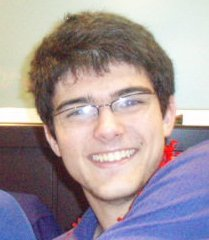
\includegraphics[scale=0.4,bb=0 100 200 300]{personal_image.jpg} & 
\raisebox{-\totalheight}{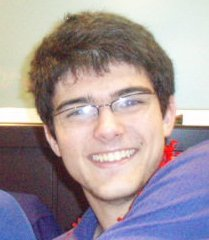
\includegraphics[width=0.2\textwidth,bb=0 0 204 270]{personal_image.jpg}} & \begin{itemize}
\item Av./ Jaume Recoder, 62-64, 4º-4ª, 08301, Mataró
\item Telf.: 636572817
\item Correo: gabrieldelacal9@gmail.com
\item Sexo: Hombre
\item Fecha de nacimiento: 06/04/1990
\item Nacionalidad: española
\end{itemize} \\
\end{tabular}
%\end{center}

\subsection*{Objetivos profesionales}
\begin{itemize}
\item Ingeniería Industrial  
\item Máster universitario UPC Automática y Robótica
\item Doctorado en Automática, Robótica y Visión
\end{itemize}

\subsection*{Educación y formación}

\begin{itemize}
\item Bachillerato tecnológico.
\item Iniciados los estudios de Ingeniería Industrial. Actualmente trabajando en el Proyecto Final de Carrera.
\item Becario en el departamento ESAII durante un periodo de 6 meses en la implementación de controles.
\end{itemize}

\textbf{Lengua materna:} español \hspace*{3cm} \textbf{Otros idiomas: Catalán} \\

\textbf{Permiso de conducir:} B1

\end{document}